\section{System Architecture}

%------- UML System Architecture
\begin{figure}[H]
	\centering
	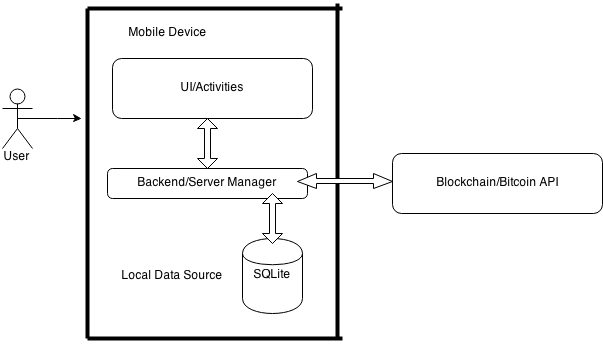
\includegraphics[scale=0.5]{../diagrams/systemArch.png}
	\caption{System Architecture UML}
\end{figure}

%--------Architecture Overview
\textbf{Architecture Overview:}\\
The application will be accessed and stored on an Android phone.  The user will interact with application using touch screen.\\
\begin{itemize}
\item Environment is mobile, can be used anywhere 
\item Users will have an existing bitcoin account(s)
\item Main functions consist of storing and organizing bitcoin wallet(s) information and displaying data
\item Input is users bitcoin account(s), output is data organization and customization\\
\end{itemize}

%--------Logical Overview
\textbf{Logical Overview:}\\

\begin{itemize}
\item Utilizing Android OS on mobile phones (rev to be determined), developing in Android SDK framework using JAVA
\item Data storage will be local, utilizing SQLite
\item Data gathered form account(s) using blockchain and bitcoin API
\item IDE will Google's Android Studio\\
\end{itemize}
	
%-------- UI/Activities Description
\textbf{UI/Activities:}\\
\begin{itemize}
\item Will be designed using Android SDK standards kn XML mark-up 
\item Purpose provides interaction with end user
\item Interactions include end user input and data binding with back-end/server manager\\
\end{itemize}

%--------- Back-end/Server Description
\textbf{Back-end/Server manager:}\\
\begin{itemize}
\item Will be designed using Android SDK standards in JAVA
\item Purpose provides interaction between database, blockchain, bitcoin API, and UI/Activities
\item Data binding will occur in this area
\item Interactions include data management, activities controller, and external data management\\
\end{itemize}

%---------- SQLite Description
\textbf{SQLite Database:}\\
\begin{itemize}
\item Will be designed using an undecided SQLite tool utilizing sql queries and statements 
\item Purpose provides data storage and management for the application
\item Interactions include Back-end/Server communication for queries and storage\\
\end{itemize}

%----------- Blockchain/Bitcoin API Description
\textbf{Blockchain/Bitcoin:}\\
\begin{itemize}
\item Will be not need to be designed. Will be managed by Back-end/Server
\item Purpose is to provide data and information from blockchain and user's existing bitcoin account(s)
\item Interactions will occur with Back-end/Server\\
\end{itemize}
